\let\negmedspace\undefined
\let\negthickspace\undefined
\documentclass[journal]{IEEEtran}
\usepackage[a5paper, margin=10mm, onecolumn]{geometry}
%\usepackage{lmodern} % Ensure lmodern is loaded for pdflatex
\usepackage{tfrupee} % Include tfrupee package

\setlength{\headheight}{1cm} % Set the height of the header box
\setlength{\headsep}{0mm}     % Set the distance between the header box and the top of the text

\usepackage{gvv-book}
\usepackage{gvv}
\usepackage{cite}
\usepackage{amsmath,amssymb,amsfonts,amsthm}
\usepackage{amsmath}
\usepackage{algorithmic}
\usepackage{graphicx}
\usepackage{textcomp}
\usepackage{xcolor}
\usepackage{txfonts}
\usepackage{listings}
\usepackage{enumitem}
\usepackage{mathtools}
\usepackage{gensymb}
\usepackage{comment}
\usepackage[breaklinks=true]{hyperref}
\usepackage{tkz-euclide} 
\usepackage{listings}
% \usepackage{gvv}                                        
\def\inputGnumericTable{}                                 
\usepackage[latin1]{inputenc}                                
\usepackage{color}                                            
\usepackage{array}                                            
\usepackage{longtable}                                       
\usepackage{calc}                                             
\usepackage{multirow}                                         
\usepackage{hhline}                                           
\usepackage{ifthen}                                           
\usepackage{lscape}
\usepackage{circuitikz}
\tikzstyle{block} = [rectangle, draw, fill=blue!20, 
    text width=4em, text centered, rounded corners, minimum height=3em]
\tikzstyle{sum} = [draw, fill=blue!10, circle, minimum size=1cm, node distance=1.5cm]
\tikzstyle{input} = [coordinate]
\tikzstyle{output} = [coordinate]


\begin{document}

\bibliographystyle{IEEEtran}
\vspace{3cm}

\title{4.8.14}
\author{AI25BTECH11018-Hemanth Reddy}
 \maketitle
% \newpage
% \bigskip
{\let\newpage\relax\maketitle}

\renewcommand{\thefigure}{\theenumi}
\renewcommand{\thetable}{\theenumi}
\setlength{\intextsep}{10pt} % Space between text and floats


\numberwithin{equation}{enumi}
\numberwithin{figure}{enumi}
\renewcommand{\thetable}{\theenumi}

\textbf{Question:}\\

Find the area of the region


$
\{(x,y) : 0 \leq y \leq x^2, 0 \leq y \leq x+2, -1 \leq x \leq 3\}.
$

\textbf{Solution:}\\

The parabola $ y = x^2 $ can be written as\\
\begin{center}
    $y - x^2 = 0$
\end{center}


or, in conic matrix form:
\begin{align}
    \vec{x}^T V \vec{x} + 2\, \vec{u}^T \vec{x} + f = 0,
\end{align}



\begin{align}
    \vec{V} = \myvec{
-1 & 0 \\
0 & 0
}, \quad
\vec{u} = \myvec{
0 \\ \frac{1}{2}
}, \quad
f = 0.
\end{align}



% Line: y = x + 2
The line \( y = x + 2 \) can be written as\\
\begin{center}
    x - y + 2 = 0,
\end{center}


The General Equation of a Line:
\begin{equation}
    \vec{x} = k\vec{m} + \vec{h}
\end{equation}
On comparing, we get:
\begin{equation}
    \vec{m} = \myvec{1 \\ 1}, \, \vec{h} = \myvec{0 \\ 2}
\end{equation}

The Intersection of the given conic with the given line can be written as:
\begin{equation}
    \vec{x}_i = \vec{h} + k_i\vec{m}
\end{equation}

\begin{equation}
    where, \, k_i = \left( \dfrac{1}{\vec{m}^\top\vec{V}\vec{m}} \right) \left( 
    -\vec{m}^\top(\vec{V}\vec{h}+\vec{u}) \, \pm \, \sqrt{[\vec{m}^\top(\vec{V}\vec{h}+\vec{u})]^2 - g(h)(\vec{m}^\top\vec{V}\vec{m})} \right) 
\end{equation}

Let $\vec{K} = \myvec{k_1 \\ k_2}$\\



The Solution Matrix can be expressed as: 
\begin{equation}
    \vec{X} = \myvec{\vec{h} & \vec{m}}\myvec{\vec{1} & \vec{k}}^\top
\end{equation}

Therefore, The points of intersection are:
\begin{equation}
    \vec{x}_1 = \myvec{-1 \\ 1} \quad \& \quad \vec{x}_2 = \myvec{2 \\4}
\end{equation}


From Fig.0.1, the required area is given by:
\begin{equation}
    \int_{-1}^{2} [(x+2) - (x^2)] \,dx = \int_{-1}^{2} [2 + x -x^2] \,dx
\end{equation}

\begin{equation}
 \int_{-1}^{2} [x^2] \,dx + \int_{2}^{3} [x+2] \,dx  = \dfrac{15}{2} = 7.5 \, sq.units   
\end{equation}

\begin{align*}
\boxed{\text{Therefore, the required area is 7.5 sq.units.}}
\end{align*}



\begin{figure}[H]
    \centering
    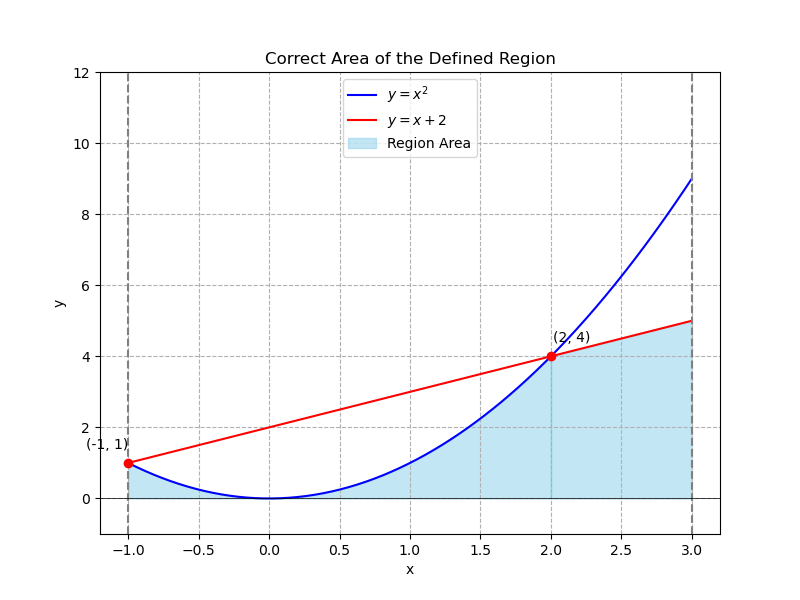
\includegraphics[width=0.8\linewidth]{figs/plot.png}
    \caption{}
    \label{fig:placeholder}
\end{figure}

\end{document}























